\documentclass[11pt]{article}

\usepackage{url}
\usepackage{hyperref}
\usepackage{graphicx}
\usepackage{upquote}
\setlength{\parskip}{0.5cm plus4mm minus3mm}

\textwidth=6.4in
\textheight=8.5in
\hoffset=-0.7in
\voffset=-0.7in

\setlength{\parindent}{0cm} 

\newcommand{\Yfun}{Y}

\hyphenation{Text-Wrangler}

\title{Chapter 1: Introduction to Spherical Harmonics}
\author{The Slepian Working Group}

\begin{document}
\maketitle

\section{Initialization}

Start Matlab or Octave and switch to the folder \verb+Slepian+

To initialize the Slepian software in Matlab, run

\qquad \verb+initialize+

To initialize the Slepian software in Octave, run

\qquad \verb+initialize_octave+

The first time you run \verb+initialize_octave+, it will download and install
missing packages. This will take a few minutes. Make sure you have
internet access. 

\subsection{Additional considerations for Octave}

If you are running Octave and your figures further on in this tutorial
look bad, then you may want to switch the graphics package Octave
uses. Try for example

\qquad \verb+graphics_toolkit('fltk')+

or

\qquad \verb+graphics_toolkit('gnuplot')+

or

\qquad \verb+graphics_toolkit('qt')+

When you are displaying a lot of output, Octave usually shows this
step by step. This is a bit annoying. We'll turn this off by running

\qquad \verb+more off+

You will need to run all of these initializations every time you start
Octave.



\section{Testing the software}\label{testing}
To check if the software installed correctly you can run a few demos
using the function \verb+demos_slepian_golf+

\qquad \verb+help demos_slepian_golf+

This will show you a description of what the program does. For
example, try

\qquad \verb+demos_slepian_golf(6)+

This will calculate and plot a single gradient vector Slepian function
for Eurasia and maximum spherical-harmonic degree $L=10$. You will
learn later in this tutorial what the spherical-harmonic degree is.
We leave the tutorial for gradient vector Slepian functions for a
later time. If you are interested you can check out for example the
article
\href{https://doi.org/10.1007/978-3-642-27793-1_64-2}{``Potential-field
  estimation using scalar and vector Slepian functions at satellite
  altitude''} (doi: \verb+10.1007/978-3-642-27793-1_64-2+) or the information
including links on the website \url{www.alainplattner.net}.


\section{Introduction to spherical harmonics}

Spherical harmonics are a counterpart to monomials (building blocks of
polynomials, the ``wiggly'' lines) but on the sphere. Remember that
polynomials were always sums of monomials multiplied by some
numbers. For example $3x^2 - 20.95x + 5.11113$ is a \emph{polynomial}
consisting of the \emph{monomials} $x^2$, $x$, and $1$ multiplied by
the \emph{coefficients} $3, -20.95, 5.1113$ and then summed
up. Spherical harmonics do exactly the same. Each of them has a
degree, we multiply them with coefficients and then sum them up. One
thing that is different is that besides having a degree, spherical
harmonics also have an order. This is because they live on a sphere
which is a surface and therefore has two directions in which it can
``wiggle''.

Here we denote spherical harmonics with the capital letter $\Yfun$
followed by its degree $l$ and its order $m$ as indices. Both degree
$l$ and order $m$ are integers. The degree $l$ is 0 or greater whereas
the order can be positive, zero, or negative. So we generally write
$\Yfun_{l\,m}$. For example for degree 4 and order 2 it will be
$\Yfun_{4\,2}$ (note the small gap between 4 and 2). The \emph{degree}
$l$ of a spherical harmonic says, how many zero-crossing lines it has
in total. The \emph{order} $m$ of a spherical harmonic says how many
of the zero-crossings are perpendicular to the equator. The sign of
the order says if one of the zero-crossings is along the
prime-meridian (negative order $m$) or if the maximum value is on the
prime meridian (positive order $m$). From this explanation it is clear
that the order $m$ must always be equal or smaller to the degree $l$
(there can't be more zero-crossings perpendicular to the equator than
there are zero-crossings altogether).

Let's look at a few examples. To make it easier to visualize the
spherical harmonics, I am plotting them on a sphere and in Mollweide
projection over Earth's map. $\Yfun_{0\,0}$ is just a constant number
over the entire planet. That's a bit boring so I won't plot it here.

\begin{figure}%[H]
\centering 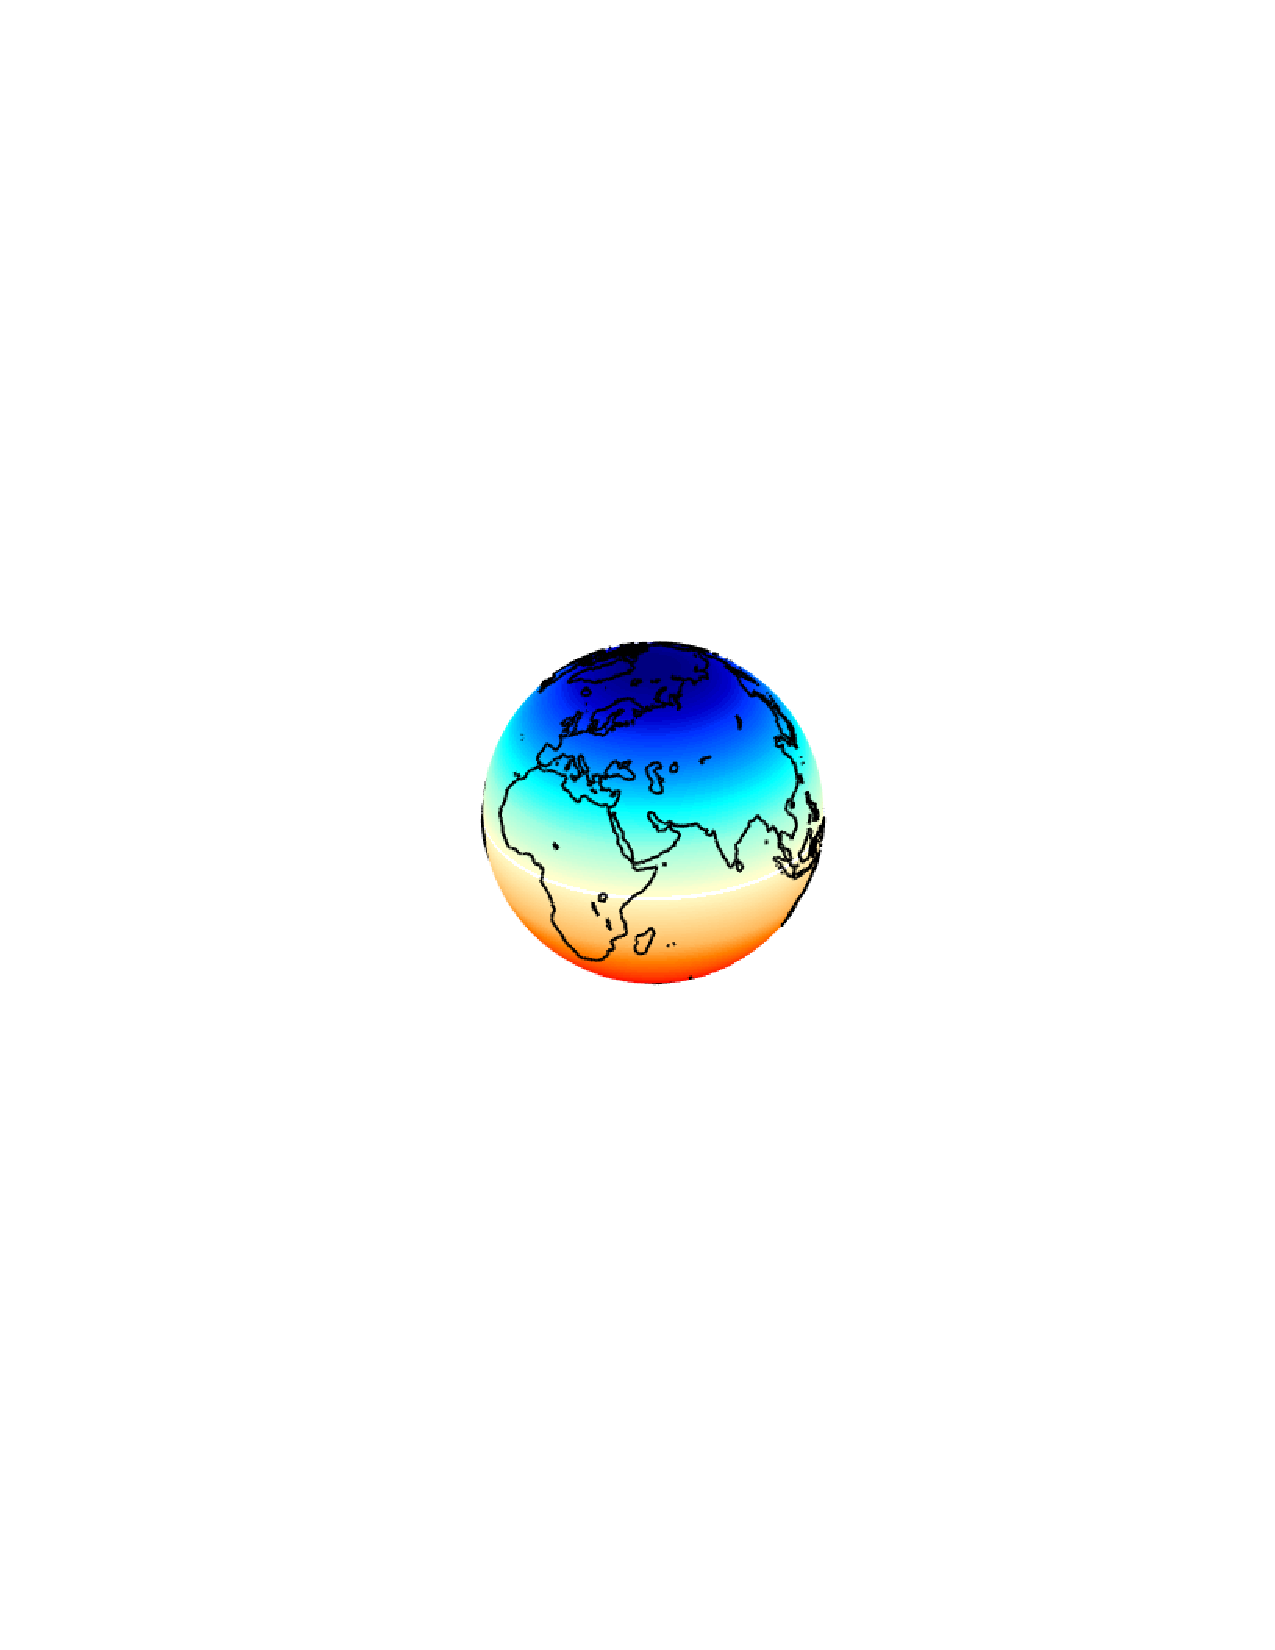
\includegraphics[width=0.39\textwidth,trim = 7cm 10cm 7cm
  10cm, clip]{figures/Fig1} 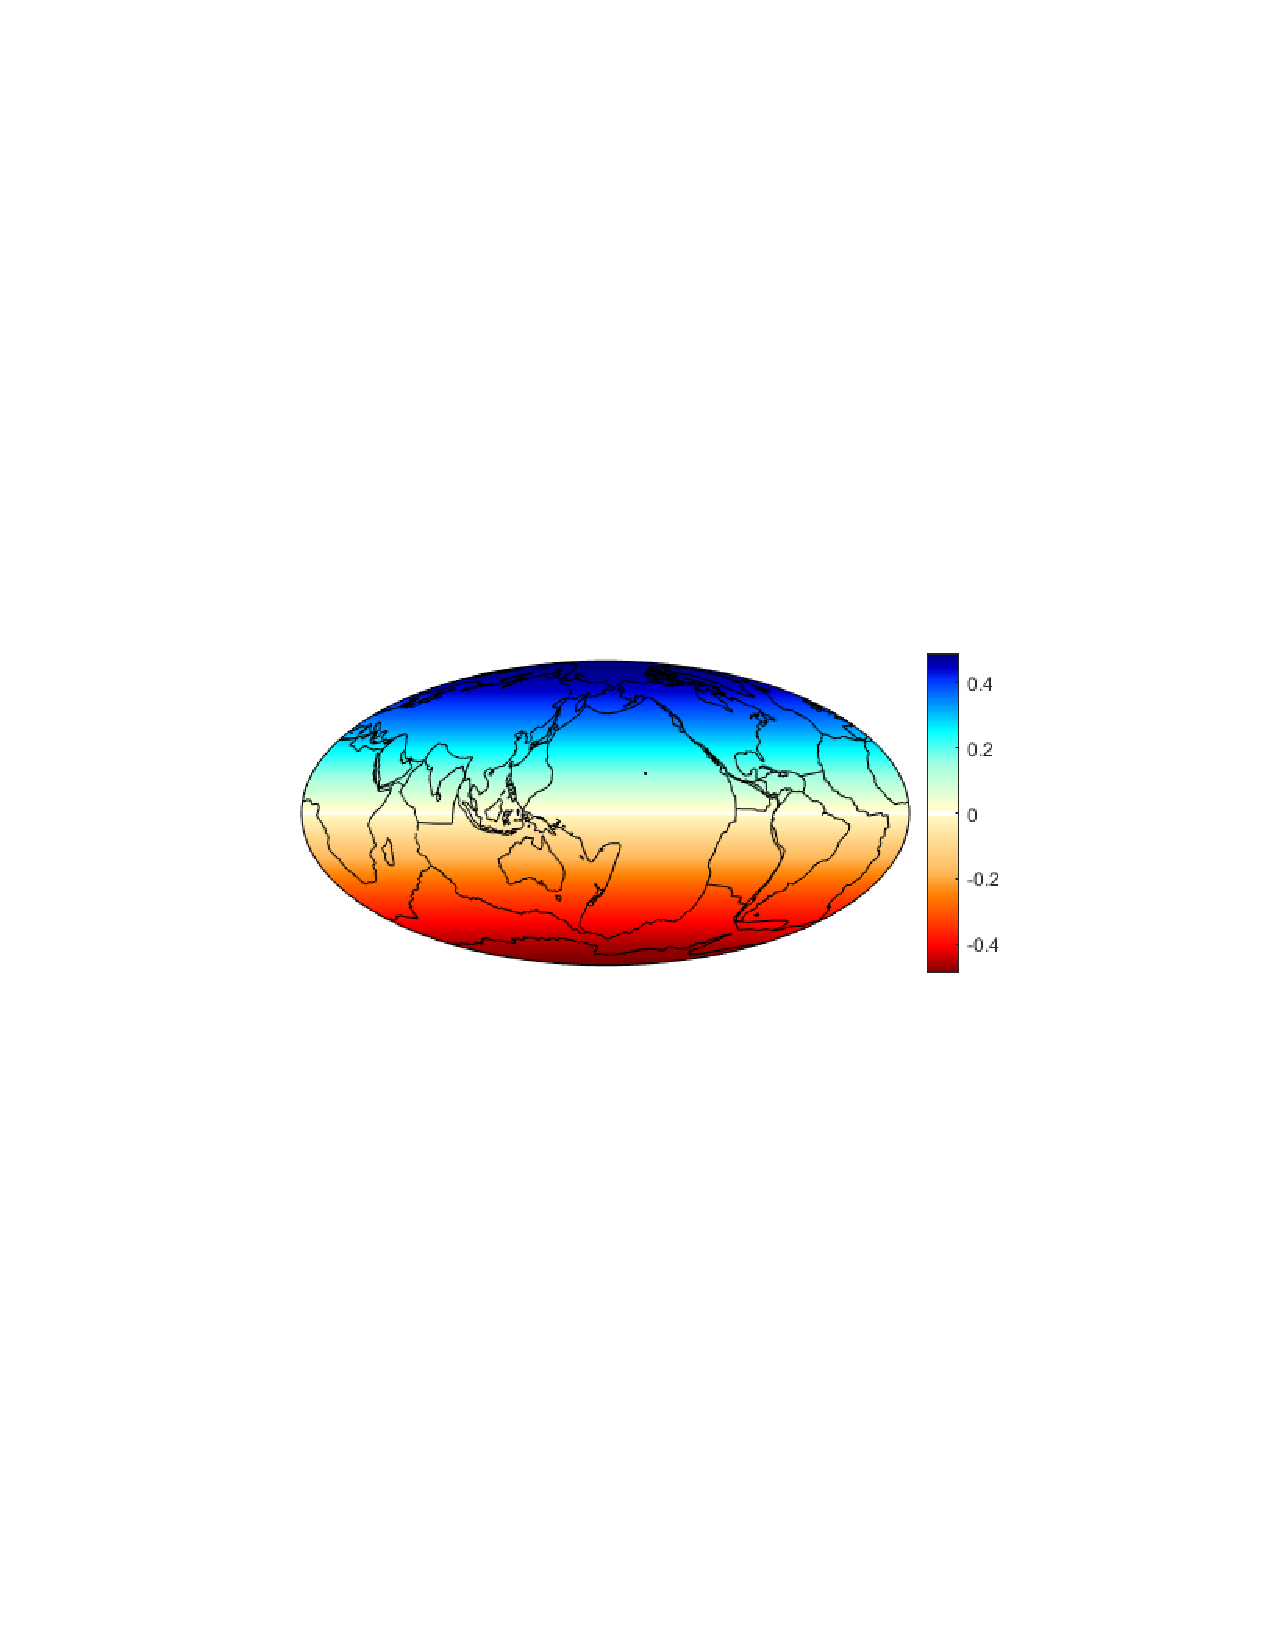
\includegraphics[width=0.6\textwidth,trim =
  3cm 9cm 3cm 10cm, clip]{figures/Fig1bar}
\caption{This is spherical harmonic $\Yfun_{1\,0}$. It's a dipole with
  its north pole over the geographical North Pole and its south pole
  over the geographical South Pole. In the left panel I am plotting it
  over a sphere, in the right panel I am using Mollweide projection}
\label{Y10fig}
\end{figure}

%\newpage
\begin{figure}%[H]
\centering \includegraphics[width=0.39\textwidth,trim = 7cm 10cm 7cm
  10cm, clip]{figures/Y1m1} \includegraphics[width=0.6\textwidth,trim
  = 3cm 9cm 3cm 10cm, clip]{figures/Y1m1_Mol}
\caption{This is spherical harmonic $\Yfun_{1\,-1}$. It's a dipole
  with its north pole over the Pacific and its south pole over
  Africa. In the left panel I am plotting it over a sphere, in the
  right panel I am using Mollweide projection.}
\label{Y1m1fig}
\end{figure}
 
\begin{figure}[ht!]
  \centering \includegraphics[width=0.39\textwidth,trim = 7cm 10cm 7cm
    10cm, clip]{figures/Y11} \includegraphics[width=0.6\textwidth,trim =
    3cm 9cm 3cm 10cm, clip]{figures/Y11_Mol}
  \caption{This is spherical harmonic $\Yfun_{1\,1}$. It's a dipole with
    its north pole over the Indian Ocean and its south pole over Central
    America. In the left panel I am plotting it over a sphere, in the
    right panel I am using Mollweide projection.}
  \label{Y11fig}
\end{figure}

\textbf{Question:} How can we make a dipole with its south pole over
the geographical North Pole and its North pole over the geographical
South Pole?


I made these plots using our codes that you just installed. Once you
chose a degree $l$ and an order $m$, you must select a plotting
grid. Let's make a pixel every half degree. From your Octave tutorial
you remember that

\qquad \verb+theta=-90:0.5:90;+

Sets up such a vector for the latitudes and 

\qquad \verb+phi=0:0.5:360;+

for the longitudes. We will use the function \verb+ylm.m+ to
calculate spherical-harmonic values on the sphere on the grid we just
defined. Notice that the symbol \verb+l+ is the letter $l$. Run

\qquad \verb+l=3+ 

and 

\qquad \verb+m=-2+

and then 

\qquad \verb+Y3m2=ylm(l,m,pi/180*(90-theta),pi/180*phi);+

This will calculate the values of $\Yfun_{lm}$ for your chosen $l$ and
$m$ on the grid you defined with latitudes \verb+theta+ and longitudes
\verb+phi+. We need the factors $\pi/180$ because the function
\verb+ylm.m+ requires the grid in radians and we need the $90-$
\verb+theta+ because the function \verb+ylm.m+ works with colatitudes
instead of latitudes.

To plot the resulting evaluated spherical harmonic \verb+Y3m2+ on a
Mollweide projection, run
  
\qquad \verb+plotplm(Y3m2,pi/180*phi,pi/180*theta,1)+

Let's change the color to a bit a nicer color scheme, run

\quad \verb+kelicol(1)+


To plot the resulting evaluated spherical harmonic on a rotatable
sphere, you need to first open a new figure or close the old one and
then run

\qquad \verb+plotplm(Y3m2,pi/180*phi,pi/180*theta,2)+

\textbf{Exercise:} Reproduce figures \ref{Y10fig}, \ref{Y1m1fig}, and \ref{Y11fig}. Plot different spherical harmonics for different degrees and orders. Plot sums of spherical harmonics. Plot linear combinations of spherical harmonics. How does for example \\{$4\Yfun_{3\,1} - 0.2\Yfun_{1\,-1} +2\Yfun_{5\,-2}$} look like?

If it looks like in figure~\ref{MixY}, then your programing was
correct.

\begin{figure}%[H]
  \centering
  \includegraphics[width=0.7\textwidth,trim = 3cm 9cm 3cm 10cm, clip]{figures/mixY}
  \caption{Linear combination of spherical harmonics $4\Yfun_{3\,1} - 0.2\Yfun_{1\,-1} +2\Yfun_{5\,-2}$ in Mollweide projection}
  \label{MixY}
\end{figure}

What we learn from this is that even though the individual spherical
harmonics look very regular with their zero-crossings either parallel
or perpendicular to the equator, linear combinations of spherical
harmonics can look very arbitrary. In fact, every reasonably behaved
function on the sphere (no infinite values and no sudden jumps, etc.)
can be expressed as a linear combination of spherical harmonics. For
some we might need spherical harmonics with very high degrees.

\textbf{Exercise:} Make your own linear combination of spherical
harmonics. Play around with the degrees and coefficients. Can you make
up some shape in your mind that you want to draw with spherical
harmonics and then reproduce it?

Calculating spherical harmonics individually, multiplying them with
coefficients, and then summing them up is cumbersome. Luckily, our
software allows us to do this more efficiently. Instead of just
calculating a single spherical harmonic we can calculate all of them
up to a any degree $L$ we choose. Run for example

\quad \verb+L=10+

and then

\quad \verb+Y=ylm([0 L],[],pi/180*(90-theta),pi/180*phi);+

This will calculate a matrix \verb+Y+ in which each row represents an
evaluated spherical harmonic. the rows are ordered in what we call
here the \emph{addmout} format. This is an informal term used within
the software suite and is not generally used in the community. Addmout
means the following ordering for the (degree/order) pairs: (0/0),
(1/-1), (1/0), (1/1), (2/-2), (2/-1), etc. This means that the
spherical harmonic with degree 2 and order 1 is in the 8th row of the
matrix \verb+Y+.
   
\textbf{Question:} In which row is degree 3, order -2? Which
degree/order pair do we find in row 20?

If we now have a vector of coefficients that we call \verb+c+, then we
can calculate the linear combination of the spherical harmonics
evaluated in matrix \verb+Y+ with the coefficients in vector \verb+c+
using matrix-vector multiplication. For a maximum spherical harmonic
degree $L$ there are $(L+1)^2$ spherical harmonics including all
degrees between 0 and $L$ and all corresponding orders.  We can
calculate a random row vector with the correct length by running

\quad \verb!c=randn(1,(L+1)^2);!
   
and evaluate the linear combination of the spherical harmonics as

\quad \verb!F=c*Y;!

The linear combination \verb!F! has the form of a vector. We need to
put it into the right shape by running

\quad \verb!Fp=reshape(F,length(theta),length(phi));!

Plot this function with the command we have seen before

\qquad \verb+plotplm(Fp,pi/180*phi,pi/180*theta,1)+

\textbf{Question:} Why are there $(L+1)^2$ spherical harmonics for
degrees 0 to $L$ and all coprresponding orders?

\textbf{Question:} Why does the matrix vector multiplication
\verb!F=c*Y;! calculate a linear combination of the spherical
harmonics with the corresponding coefficients in \verb+c+?


\textbf{Exercise:} If I give you a random list of data point values
together with their locations, can you find a way to calculate
best-fitting spherical-harmonic coefficients? Remember least-squares
fitting.


\end{document}
